\setboolean{IsHalfPage}{false}%
\setboolean{IsHalfPageLeftCol}{false}%
\setboolean{IsHalfPageRightCol}{false}%
\def\ChapterTitle{%
	NURTURE
}
\def\ChapterUrl{%
	https://arnottferels.github.io/work/nurture
}
\def\ChapterDescription{%
	Nutrient for future Singapore
}
\def\ChapterDetailsLine{%
	Master's Design Studio 2 -- 2022 | Urban Housing Research; Apartment Design; Sustainable Design | Singapore
}
\def\ChapterDetailsTabular{%
	\begin{tabular}{@{}ll}
		\textbf{Type}          & International Student Competition by Designing Resilience in Asia (DRIA) \& TU Darmstadt            \\
		\textbf{Contributions} & Conceptual, Formal analysis, Software (3D modeling and simulation), Housing design \& Visualization \\
		\textbf{Software}      & Rhino \& Grasshopper                                                                                \\
		\textbf{Collaborators} & Fikri Nur Khalid, Ekky Maulidin, Citra Destianti, Farelio Artha \& Hasrul Nurliansyah               \\
		\textbf{Advisor}       & M. Prasetiyo Effendi Yasin \& Roro Diah Asih Purwaningrum                                           \\
		\textbf{URL}           & \textcolor{blue}{\footnotesize\texttt{\href{\ChapterUrl}{\ChapterUrl}}}                             \\
	\end{tabular}
}
\def\ChapterAbstract{%
	This project aims to revitalize Singapore's urban environment, tackling critical issues like food security and environmental sustainability, which are primary concerns in the country. By integrating education-focused communities with advanced technology, the pond-centric design, especially in housing placement, promotes sensory learning within the Transit-Oriented Development (TOD) framework. The proposed design advocates for a self-sufficient strategy through both public and private housing, contributing significantly to Singapore's 2030 goal of attaining 30\% food self-sufficiency. This initiative marks a comprehensive shift towards sustainable living for future residents of Singapore.
}
\def\ChapterFrontmatter{%
	\chapter*{\ChapterTitle}\addcontentsline{toc}{chapter}{\ChapterTitle}
	\ChapterSetTocAddData{\ChapterDetailsLine}
	\ChapterSetDetailsData{\ChapterDescription}{\ChapterDetailsLine}{\ChapterDetailsTabular}
	\RuleAbstract%
	\ChapterAbstract
}
\StartTwoColumnLayout
\ChapterFrontmatter
\vspace*{0.75cm}%
\section*{%
  Background
 }
\setlength{\ColumnGap}{1cm}
\setlength{\MinipageGap}{1cm}
\setlength{\HalfLineWidth}{0.5\linewidth}
\setlength{\MinipageAWidth}{\dimexpr ((0.2\HalfLineWidth) - (0.5\ColumnGap))\relax}
\setlength{\MinipageBWidth}{\dimexpr (\HalfLineWidth - \MinipageAWidth - \MinipageGap - (0.5\ColumnGap))\relax}
\setlength{\columnsep}{\ColumnGap}%
\begin{multicols}{2}
	\begin{minipage}{\MinipageAWidth}
		\begin{tikzpicture}
			\draw[color=SpringGreen4, line width=4pt]
			(90:2cm) arc[start angle=90, end angle=414, radius=1cm];
			\node at (90:1cm) {\Large 90\%};
		\end{tikzpicture}
	\end{minipage}
	\hspace{\MinipageGap}%
	\begin{minipage}{\MinipageBWidth}
		By 2030, Singapore aims to produce 30\% of its own food, reducing its reliance on the current 90\% imported.
	\end{minipage}
	\columnbreak%
	\begin{minipage}[t]{\linewidth}
		\begin{minipage}{\MinipageAWidth}
			\begin{tikzpicture}
				\draw[color=SpringGreen4, line width=4pt]
				(90:2cm) arc[start angle=90, end angle=90-40.4*3.6, radius=1cm];
				\node at (90:1.1cm) {\Large 40.4\%};
			\end{tikzpicture}
		\end{minipage}
		\hspace{\MinipageGap}%
		\begin{minipage}{\MinipageBWidth}
			In Singapore, using 151~liters of water per day compared to the United States' 375~liters, there are plans to increase water recycling from 40\%~to~50\% by 2030 for sustainability. By 2030, Singapore aims to produce 30\% of its own food, reducing its reliance on the current 90\% imported.
		\end{minipage}
	\end{minipage}
\end{multicols}
\vfill
\columnbreak%
\section*{%
  Issues \& Strategies
 }
\setlength{\MinipageGap}{1cm}
\setlength{\MinipageAWidth}{0.575\linewidth}
\setlength{\MinipageBWidth}{\dimexpr\linewidth - \MinipageAWidth - \MinipageGap\relax}
\makebox[\linewidth][l]{%
	\begin{minipage}[t]{\MinipageAWidth}
		\begin{figure}[H]
	\centering
	\includesvg[width=\linewidth]{src/graphics/nurture--issues-strat.svg}
	\label{
		fig:nurture--issues-strat
	}
\end{figure}

	\end{minipage}
	\hspace{\MinipageGap}%
	\begin{minipage}[t]{\MinipageBWidth}
		NURTURE aims to create education-focused communities in new residential areas in Singapore. These communities will encourage a harmonious coexistence with nature. The concept includes Waste Water Treatment Plants (WWTP) and educational technology to match the learning preferences and environmental appreciation of Singaporeans. NURTURE is a comprehensive approach that deals with both education and the environment, aiming to instill a sense of environmental independence. Starting at the Keppel Club site, this initiative aims to inspire nationwide change towards sustainable living.
	\end{minipage}
}
\section*{%
  Design Approach
 }
\makebox[\linewidth][l]{%
	\begin{minipage}[t]{\dimexpr \MinipageAWidth}
		\begin{figure}[H]
	\centering
	\includesvg[width=\linewidth]{src/graphics/nurture--design-approach.svg}
	\label{
		fig:nurture--design-approach
	}
\end{figure}

	\end{minipage}
	\hspace{\MinipageGap}%
	\begin{minipage}[t]{\MinipageBWidth}
		To promote farming and assist people in becoming accustomed to it, the site incorporates specific areas that blend education and entertainment, referred to as `Eduagritainment.' This term merges Education, Agriculture, and Entertainment, emphasizing the integration of these elements on the site.
	\end{minipage}
}
\end{multicols}
\section*{%
  Design Process
 }
\newlength{\FigureNurtureProcessBaseImageSize}
\newlength{\FigureNurtureProcessFinalImageSize}
\newlength{\FigureNurtureProcessImageGap}
\def\FigureNurtureImagesPerColumn{5}
\edef\FigureNurtureProcessColumnGapCount{%
	\number\numexpr\FigureNurtureImagesPerColumn - 1\relax}
\newcount\tempnum
\tempnum=\numexpr10000 / \FigureNurtureImagesPerColumn\relax
\edef\FigureNurtureProcessBaseImageSize{0.\the\tempnum}
\setlength\FigureNurtureProcessImageGap{0.5cm}
\setlength\FigureNurtureProcessFinalImageSize{%
	\dimexpr\FigureNurtureProcessBaseImageSize
	\dimexpr(
	\paperwidth
	-\PaperLeftMargin
	-\PaperRightMargin
	-\FigureNurtureProcessColumnGapCount\FigureNurtureProcessImageGap)
	\relax
}
\newcommand{\FigureNurtureProcessDataForTabularFigures}[3]{%
	\begin{minipage}[t]{\FigureNurtureProcessFinalImageSize}
		#1%
		\captionof*{figure}{%
			\parbox{\FigureNurtureProcessFinalImageSize}{%
				\centering
				\textnormal{%
					\textcolor{black}{%
						#2%
						\\
					}
				}
				\scriptsize
				#3%
			}
		}
	\end{minipage}%
}
\def\Gap{\FigureNurtureProcessImageGap}%
\def\Figure{\FigureNurtureProcessDataForTabularFigures}%
\begin{table}[H]
	\centering
	\begin{tabularx}{\linewidth}{%
		@{}c@{\hspace{\Gap}}c@{\hspace{\Gap}}c@{\hspace{\Gap}}c@{\hspace{\Gap}}c@{}
		}
		\Figure{%
			\includesvg[width=\linewidth]{src/graphics/nurture--process-01.svg}
		}%
		{Context}%
		{Describing the surrounding environment and setting.}       &
		\Figure{%
			\includesvg[width=\linewidth]{src/graphics/nurture--process-02.svg}
		}%
		{River Path \& Ponds}%
		{Examining the existing river and pond features.}           &
		\Figure{%
			\includesvg[width=\linewidth]{src/graphics/nurture--process-03.svg}
		}%
		{Radiation Analysis}%
		{Studying the impact of radiation in the area.}             &
		\Figure{%
			\includesvg[width=\linewidth]{src/graphics/nurture--process-04.svg}
		}%
		{Spherical View Analysis}%
		{Evaluating the panoramic view in a spherical perspective.} &
		\Figure{%
			\includesvg[width=\linewidth]{src/graphics/nurture--process-05.svg}
		}%
		{Housing Placement}%
		{Selecting locations for residential buildings.}              \\[\dimexpr\Gap]%
		\Figure{%
			\includesvg[width=\linewidth]{src/graphics/nurture--process-06.svg}
		}%
		{Features}%
		{Identifying roads, ponds, rivers, paths, and green areas.} &
		\Figure{%
			\includesvg[width=\linewidth]{src/graphics/nurture--process-07.svg}
		}%
		{Concept: Learning by Senses (LBS)}%
		{Educational approach focused on sensory learning.}         &
		\Figure{%
			\includesvg[width=\linewidth]{src/graphics/nurture--process-08.svg}
		}%
		{Design Adjustment \& TOD}%
		{Revisiting the design using Transit-Oriented Development.} &
		\Figure{%
			\includesvg[width=\linewidth]{src/graphics/nurture--process-09.svg}
		}%
		{Water Treatment}%
		{Water purification for housing units.}                     &
		\Figure{%
			\includesvg[width=\linewidth]{src/graphics/nurture--process-10.svg}
		}%
		{Final Design}%
		{}%
	\end{tabularx}
\end{table}

\newpage
\begin{minipage}[t]{0.375\linewidth}
	\section*{%
	  Activities
	 }
	\begin{figure}[H]
	\centering
	\includesvg[width=\linewidth]{src/graphics/nurture--activities-01.svg}
	\label{
		fig:nurture--activities-01
	}
\end{figure}

	\vspace{0.5cm}
	\begin{figure}[H]
	\centering
	\includesvg[width=\linewidth]{src/graphics/nurture--activities-02.svg}
	\label{
		fig:nurture--activities-02
	}
\end{figure}

	\vspace*{\baselineskip}
	\section*{%
	  Housing Layout Plan
	 }
	\vspace*{-\baselineskip}
	\setlength{\columnsep}{0.25cm}
	\begin{multicols}{2}
		\begin{figure}[H]
	\centering
	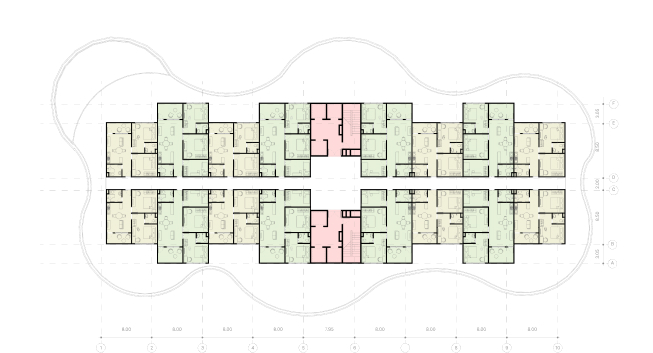
\includegraphics[width=\linewidth]{src/graphics/nurture--pub-housing-typical-floor-01.jpg}
	\caption*{%
		Public Housing (Typical Floor 1)
	}
	\label{
		fig:nurture--pub-housing-typical-floor-01
	}
\end{figure}

		\begin{figure}[H]
	\centering
	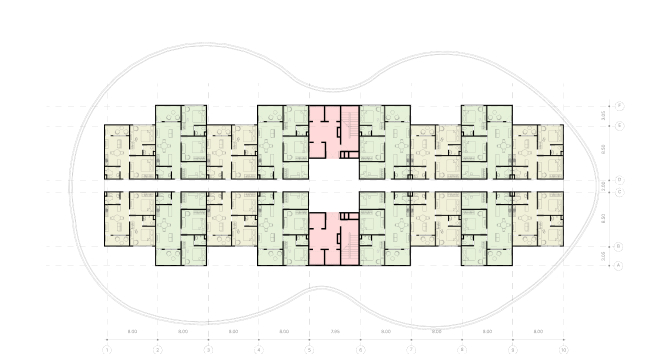
\includegraphics[width=\linewidth]{src/graphics/nurture--pub-housing-typical-floor-02.jpg}
	\caption*{%
		Public Housing (Typical Floor 2)
	}
	\label{
		fig:nurture--pub-housing-typical-floor-02
	}
\end{figure}

		\begin{figure}[H]
	\centering
	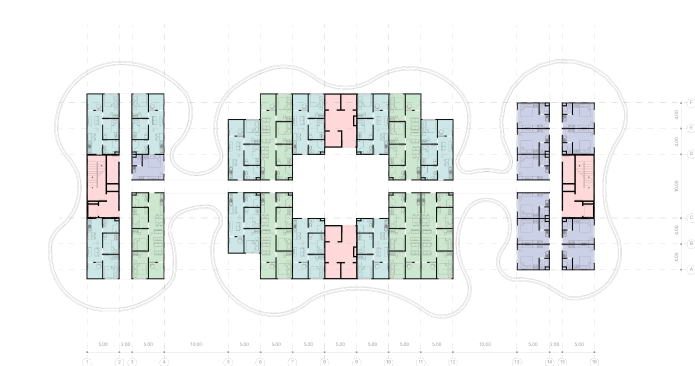
\includegraphics[width=\linewidth]{src/graphics/nurture--priv-housing-typical-floor-01.jpg}
	\caption*{%
		Private Housing (Typical Floor 1)
	}
	\label{
		fig:nurture--priv-housing-typical-floor-01
	}
\end{figure}

		\begin{figure}[H]
	\centering
	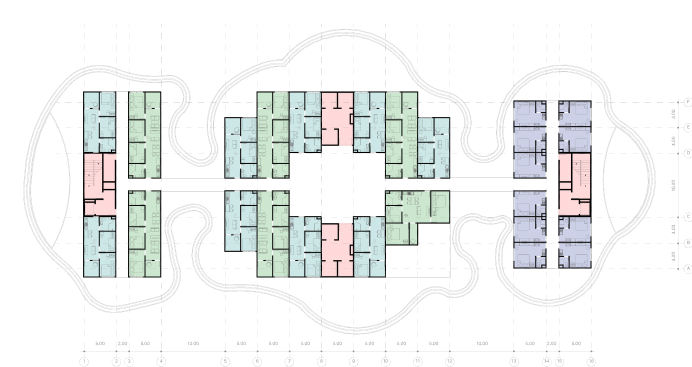
\includegraphics[width=\linewidth]{src/graphics/nurture--priv-housing-typical-floor-02.jpg}
	\caption*{%
		Private Housing (Typical Floor 2)
	}
	\label{
		fig:nurture--priv-housing-typical-floor-02
	}
\end{figure}

	\end{multicols}
	\definecolor{VerticalCirculation}{HTML}{FFDADA}
	\definecolor{Type68m2Public}{HTML}{CCE7E7}
	\definecolor{Type93m2Public}{HTML}{CCD0E7}
	\definecolor{Type20m2Private}{HTML}{CCE7CF}
	\definecolor{Type47m2Private}{HTML}{F1F0D9}
	\definecolor{Type68m2Private}{HTML}{F1F0D9}
	\newcommand{\HousingLayoutPlanLegendItem}[2]{%
		\begin{tikzpicture}
			\fill[#1] (0,0) rectangle (0.2,0.2);
		\end{tikzpicture}~\text{#2}
	}
	\def\LegendItem{\HousingLayoutPlanLegendItem}%
	\tiny
	\centering
	{%
		\LegendItem{VerticalCirculation}{Vertical Circulation} \hspace{3pt} %
		\LegendItem{Type68m2Public}{Type~68\,$\text{m}^2$ (Public)} \hspace{3pt} %
		\LegendItem{Type93m2Public}{Type~93\,$\text{m}^2$ (Public)} \hspace{3pt} %
		\LegendItem{Type20m2Private}{Type~20\,$\text{m}^2$ (Private)} \hspace{3pt} %
		\LegendItem{Type47m2Private}{Type~47\,$\text{m}^2$ (Private)} \hspace{3pt} %
		\LegendItem{Type68m2Private}{Type~68\,$\text{m}^2$ (Private)}
	}%
	\section*{%
	  Calculation
	 }
	\newcolumntype{C}[1]{>{\centering\arraybackslash}p{#1}}
	\setlength{\columnsep}{0.75cm}%
	\begin{multicols}{2}
		\noindent\begin{minipage}{\linewidth}
			\subsection*{Total Building Unit}
		\end{minipage}
		\begin{table}[H]
	\small
	\begin{tabularx}{\linewidth}{@{} p{1.2cm} X X c@{}}
		\toprule
		\textbf{Housing Type}                               & \textbf{Total\newline\ Building} & \textbf{Unit\newline\ Type} & \textbf{Total\newline\ Units} \\
		\midrule
		\multirow{3}{*}{Public}                             & \multirow{3}{*}{7}               & 1 BR                        & 2684                          \\
		                                                    &                                  & 2 BR                        & 2590                          \\
		                                                    &                                  & 3 BR                        & 1554                          \\
		\midrule
		\multirow{2}{*}{Private}                            & \multirow{2}{*}{6}               & Apartment                   & 1344                          \\
		                                                    &                                  & Condominium                 & 1344                          \\
		\midrule
		\multicolumn{3}{@{} l @{}}{\noindent\textbf{Total}} & \textbf{9526}                                                                                  \\
		\bottomrule
	\end{tabularx}
\end{table}

		\vfill
		\noindent\begin{minipage}{\linewidth}
			\subsection*{Total Area Unit per Floor}
		\end{minipage}
		\begin{table}[H]
	\small
	\begin{tabularx}{\linewidth}{@{}p{1.2cm} X X X c@{}}
		\toprule
		\textbf{Housing Type}    & \textbf{Total Floors} & \textbf{Unit\newline\ /floor} & \textbf{Unit\newline\ Type} & \textbf{Total Area\newline\ ($\textbf{m}^\textbf{2}$)} \\
		\midrule
		\multirow{3}{*}{Public}  & \multirow{3}{*}{37}   & \multirow{3}{*}{26}           & 1 BR                        & 250                                                    \\
		                         &                       &                               & 2 BR                        & 594                                                    \\
		                         &                       &                               & 3 BR                        & 490                                                    \\
		\midrule
		\multirow{2}{*}{Private} & \multirow{2}{*}{28}   & \multirow{2}{*}{16}           & Apartment                   & 893                                                    \\
		                         &                       &                               & Condominium                 & 653                                                    \\
		\bottomrule
	\end{tabularx}
\end{table}

		\vfill
	\end{multicols}
\end{minipage}
\hfill
\begin{minipage}[t]{0.6\linewidth}
	\section*{%
	  Programs
	 }
	\begin{figure}[H]
	\centering
	\includesvg[width=\linewidth]{src/graphics/nurture--programs.svg}
	\label{
		fig:nurture--programs
	}
\end{figure}

	\vfill
	\vspace*{\baselineskip}
	\section*{%
	  Perspective
	 }
	\vspace*{-\baselineskip}
	\setlength{\columnsep}{0.5cm}%
	\begin{multicols}{2}
		\begin{figure}[H]
	\centering
	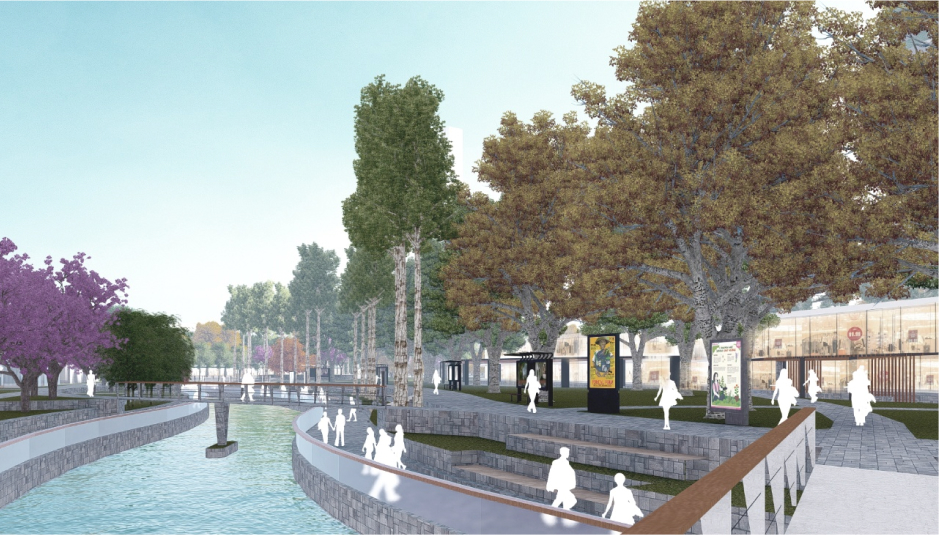
\includegraphics[width=\linewidth]{src/graphics/nurture--perspective-01.jpg}
	\vspace{-0.5\baselineskip}%
	\caption*{%
		\raggedright
		\small
		\setstretch{1.25}%
		\textcolor{black}{%
			\textnormal{%
				``The River'' blends various activities along the waterfront, market center, and hawker center, forming a lively and diverse environment.
			}
		}
	}
	\label{
		fig:nurture--perspective-01
	}
\end{figure}

		\begin{figure}[H]
	\centering
	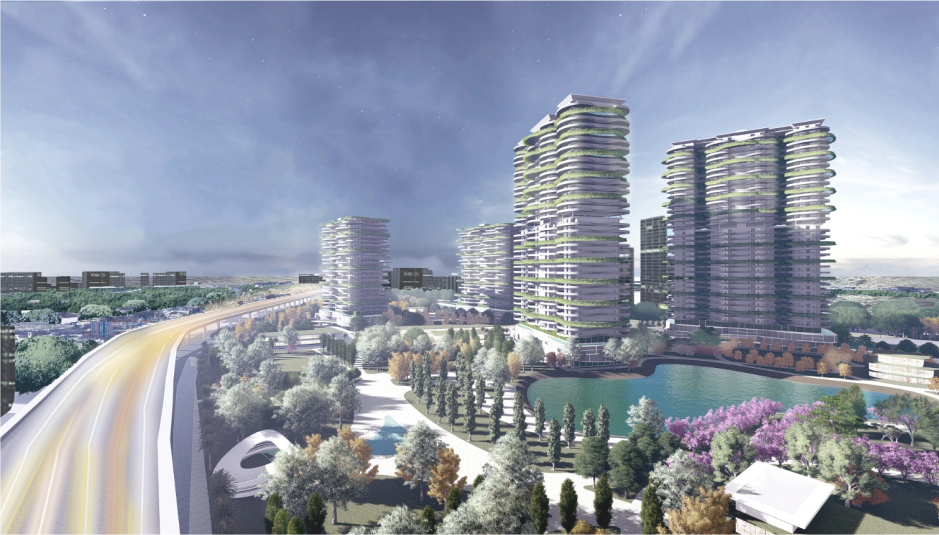
\includegraphics[width=\linewidth]{src/graphics/nurture--perspective-02.jpg}
	\vspace{-0.5\baselineskip}%
	\caption*{%
		\raggedright
		\small
		\setstretch{1.25}%
		\textcolor{black}{%
			\textnormal{%
				Aerial view -- Showcase MRT station and housing placement, integration with surroundings, emphasizing their relation to ponds. The conceptual phase prioritizes a pond-centric approach, considering the conducted environmental analysis.
			}
		}
	}
	\label{
		fig:nurture--perspective-02
	}
\end{figure}

	\end{multicols}
	\vfill
	\section*{%
	  Water Treatment Plan
	 }
	\begin{figure}[H]
	\centering
	\includesvg[width=\linewidth]{src/graphics/nurture--wwtp.svg}
	\label{
		fig:nurture--wwtp
	}
\end{figure}

\end{minipage}
\newpage
